\documentclass[12pt,a4paper]{article}
\usepackage[utf8]{inputenc}
\usepackage{amsmath}
\usepackage{amsfonts}
\usepackage{amssymb}
\usepackage{makeidx}
\usepackage{graphicx}
\usepackage[left=2cm,right=2cm,top=2cm,bottom=2cm]{geometry}

\begin{document}
\title{\textbf{Sistemas electronicos de interfaz\\EV 2.6. Construir un amplificaciòn con conexiòn darlington\\Practica 7}}
\author{Josue Natanael Orozco Nevares 18311797\\Angel Eraclio Briano Garcia 18311625\\Ing. Mecatronica\\Grado 4B}
\date{8 de noviembre del 2019}
\maketitle
\begin{figure}[h!]
\centering

\includegraphics[width=10cm]{UPCDLZMDG5783-logo.png} 
\end{figure}
\newpage

\section{Introducciòn}
En esta practica se aprendera a como poder controlar o activar un relevador industrial con una corriente de 24V con un circuito igual al de la practica 3, en el cual se divide en tres partes la primera con el boton y el optoacoplador, el segundo seria nuestro arduino 1 y el final seria el relevador industrial y el tip.


\section{Objetivo}
Activar el relevador industrial mediante la señal enviada por el arduino.

\section{Materiales}
Protoboard\\Resistencias varias\\Optoacoplador 4n25\\Cables de protoboard\\Tip 112\\Leds\\Push boton\\Laptop\\Modulo de arduino UNO\\Relevador industrial

\section{Desarrollo}
\textbf{1-} Se utilizara un circuito parecido al de la practica 3 con un optoacoplador resistencias y un boton que al momento de conectar al arduino nos de una señal de entrada.
\begin{figure}[h!]
\centering
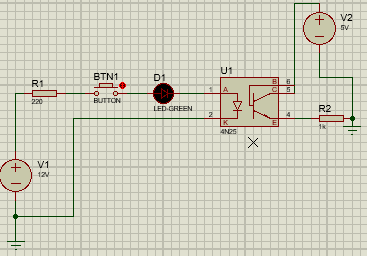
\includegraphics[scale=1]{Captura.PNG} 
\end{figure}

\textbf{2-} Se programara el modulo de arduino para que al captar la señal de entrada nos envie una de salida para que se pueda activar el relevador que esta alimentado de 24V. El cual es un circuito que recibe la señal de salida en el TIP112.
\newpage

\textbf{3-} Ya armadas las tres partes del circuito es conectar todo, la señal de entrada y la seña de salida al arduino rectificando que todo este en orden ya que si ago sale mal, el voltaje que el relevador industrial dispara de regreso puede llegar a quemar el modulo de arduino que se esta utilizando. una vez alimentado todo de 12V y 24V,con el programa ya cargado se hace la prueba de que funciona el circuito completo y que al enviar una señal de entrada la de salida hace que se active el relevador y sin ningun tipo de riesgo de que se valla a quemar algun componente.
\begin{figure}[h!]
\centering
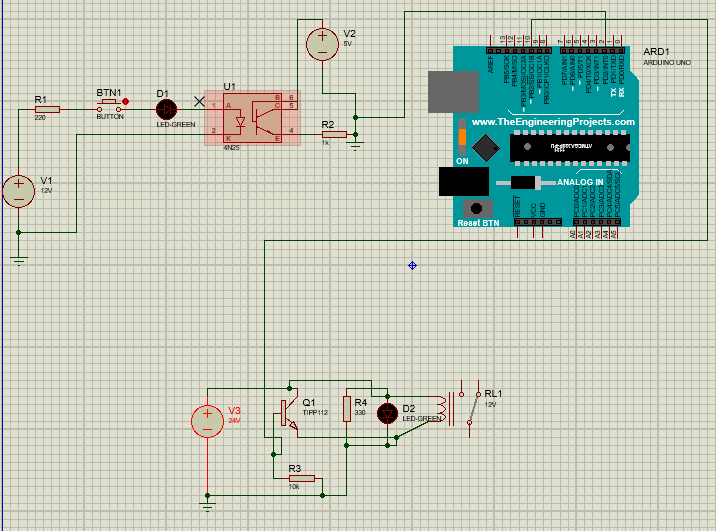
\includegraphics[scale=1]{Captura2.PNG} 
\end{figure}
\section{Conclusiòn}
Para concluir con esta practica, cabe resaltar que si no se conecta bien el TIP112 se quema, no explota solo se sobrecalienta y sale humo. Apesar de que es algo que ya habiamos realizado antes el simple hecho de saber que si algo salia mal con el relevador industrial este podia quemar el arduino, resulto ser una practica un tanto sencilla ya que casi todo el circuito ya lo habiamos armado, solo se realizaron algunas modificaciones para poder realizarlo correctamente. 

\end{document}